
\subsubsection{Administrator scenarios}
\subsubsection*{Scenario 10}
Alessandro is an administrator of the Dream system and wants to add a new data source. He connects to the administration site and login using his administrator credentials. On the administration screen he selects the “Manage data sources” section. He clicks on the button to add a new data source and inserts the source link from where the data will be recovered and clicks on the import button.
\newpage
\subsubsection*{Use case diagram}
\begin{figure}[h!]
        \centering
        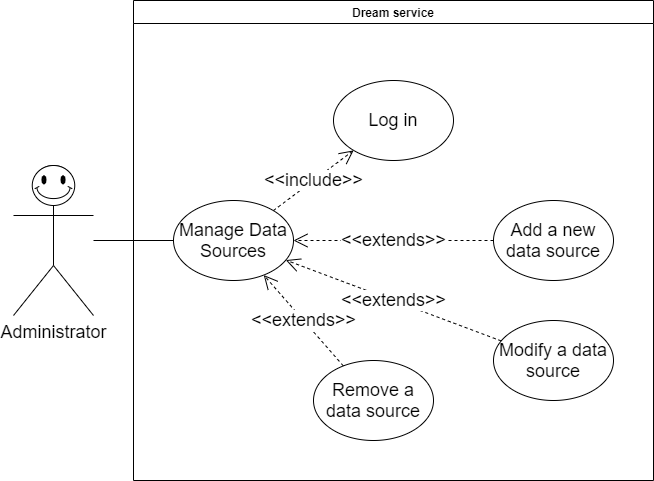
\includegraphics[scale=0.40]{images/use_cases_diagram/administrator_use_case.png}
        \caption{Use case diagram}
        \label{fig:administrator_use_case}
    \end{figure}
    \FloatBarrier
\subsubsection*{Use case tables}
\begin{longtable}{p{.25\textwidth} | p{.75\textwidth}}
\caption{Login Administrator}
        \label{tab:login_administrator}\\
        \hline
        \textbf{ID} & 19\\
        \hline
        \textbf{Name}  &  Login Administrator \\
        \hline
        \textbf{Actor}  &  Administrator\\
        \hline
        \textbf{Entry condition}  &  
        \begin{itemize}
                \item Administrator has reached the administration site
         \end{itemize}\\
        \hline
        \textbf{Input}  & Administrator's email and password\\ 
        \hline
        \textbf{Events flow} & 
        \begin{itemize}
            
                \item The system displays the login page
                \item Administrator fills the username (email) and password fields using the credential
                \item System checks the validity of the credentials inserted
                \item The system displays the precedent page or, if unavailable, the home page of the administration dashboard
                 \end{itemize}
                 \\
        \hline
        \textbf{Exit condition} & Administrator is logged in\\
        \hline
        \textbf{Exceptions} & Administrator inserts wrong credentials and clicks on “login” button. The system shows an error message inviting the Administrator to check the credentials before trying again to login\\
        \hline
       
        
    \end{longtable}
    
    \begin{figure}[h!]
        \centering
        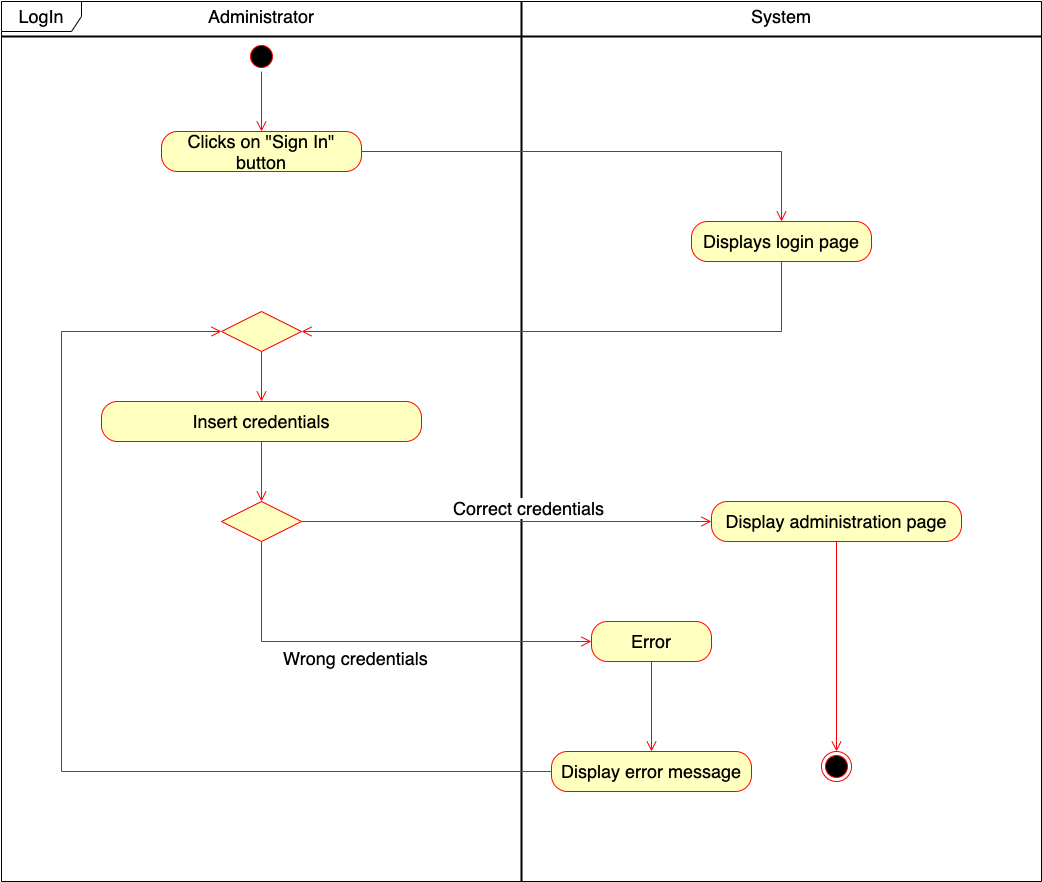
\includegraphics[scale=0.35]{images/use_cases_diagram/administrator_login.png}
        \caption{Login Administrator}
        \label{fig:administrator_login}
    \end{figure}
 \FloatBarrier   
 
 \newpage
 
\begin{longtable}{p{.25\textwidth} | p{.75\textwidth}}
    \caption{Add new data source}
        \label{tab:add_new_data_source}\\
        \hline
        \textbf{ID} & 20\\
        \hline
        \textbf{Name}  &  Add new data source \\
        \hline
        \textbf{Actor}  &  Administrator\\
        \hline
        \textbf{Input}  &  Data source to add\\
        \hline
        \textbf{Entry condition}  &  
        \begin{itemize}
                \item The Administrator is already registered in the system
                \item The Administrator is already logged in the system
                \item The Administrator is in the admin home page
         \end{itemize}\\
        \hline
        \textbf{Events flow} & 
        \begin{itemize}
                \item The Administrator selects the “Data sources” section
                \item The System opens the “Data sources” page
                \item The Administrator clicks on the button to add a new source
                \item The System render the form to add a new source
                \item The Administrator compile the form with the new data source’s origin
                \item The Administrator confirms the operation 
                 \end{itemize}
                 \\
        \hline
        \textbf{Exit condition} & The new data source is available on the site\\
        \hline
        \textbf{Exceptions} & 
        \begin{itemize}
                \item The Administrator tries to insert an unavailable source
                \item The Administrator tries to insert a data source already present in the system
                \end{itemize}
                \\
        \hline
        \textbf{Special requirements}  &  The Administrator needs to have the copyright permission to use the data source\\
        \hline
       
        
    \end{longtable}
    
    \begin{figure}[h!]
        \centering
        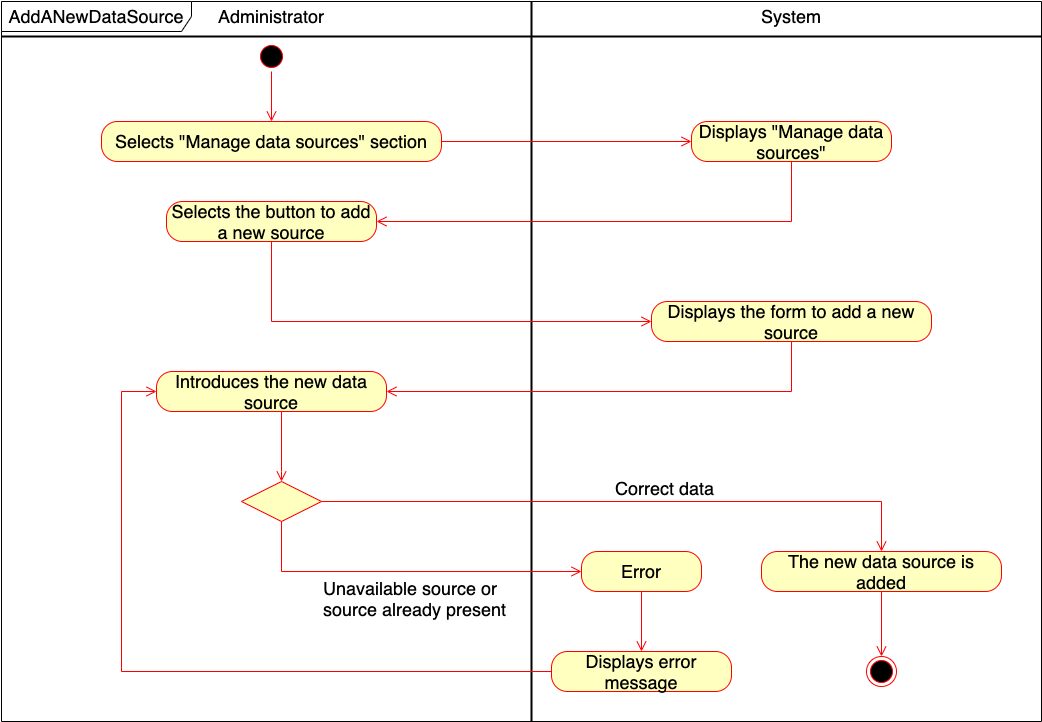
\includegraphics[scale=0.35]{images/use_cases_diagram/administrator_add_datasource.png}
        \caption{Add new data source}
        \label{fig:administrator_add_datasource}
    \end{figure}
   \FloatBarrier 
   
   \begin{longtable}{p{.25\textwidth} | p{.75\textwidth}}
     \caption{Modify a data source}
        \label{tab:modify_data_source}\\
        \hline
        \textbf{ID} & 21\\
        \hline
        \textbf{Name}  &  Modify a data source\\
        \hline
        \textbf{Actor}  &  Administrator\\
        \hline
        \textbf{Input}  &  Changes to a data source\\
        \hline
        \textbf{Entry condition}  &  
        \begin{itemize}
                \item The Administrator is already registered in the system
                \item The Administrator is already logged in the system
                \item The Administrator is in the admin home page
         \end{itemize}\\
        \hline
        \textbf{Events flow} & 
        \begin{itemize}
                \item The Administrator selects the “Data sources” section
                \item The System opens the “Data sources” page
                \item The Administrator clicks on the “Modify” button associated to the data source he wants to modify
                \item The System render a form, from which the administrator could modify some data 
                \item The Administrator modify some parameters of the selected data source
                \item The Administrator confirms the operation 
                 \end{itemize}
                 \\
        \hline
        \textbf{Exit condition} & The data source is modified and is available on the site\\
        \hline
        \textbf{Exceptions} &  
        \begin{itemize}
            \item The Administrator doesn’t confirm the operation
            \item The changes results in equivalence with another existing data source
        \end{itemize}\\
        \hline
        \textbf{Special requirements} &  The Administrator needs to have the copyright permission to use the data source\\
        \hline
       
        
    \end{longtable}

    \begin{figure}[h!]
        \centering
        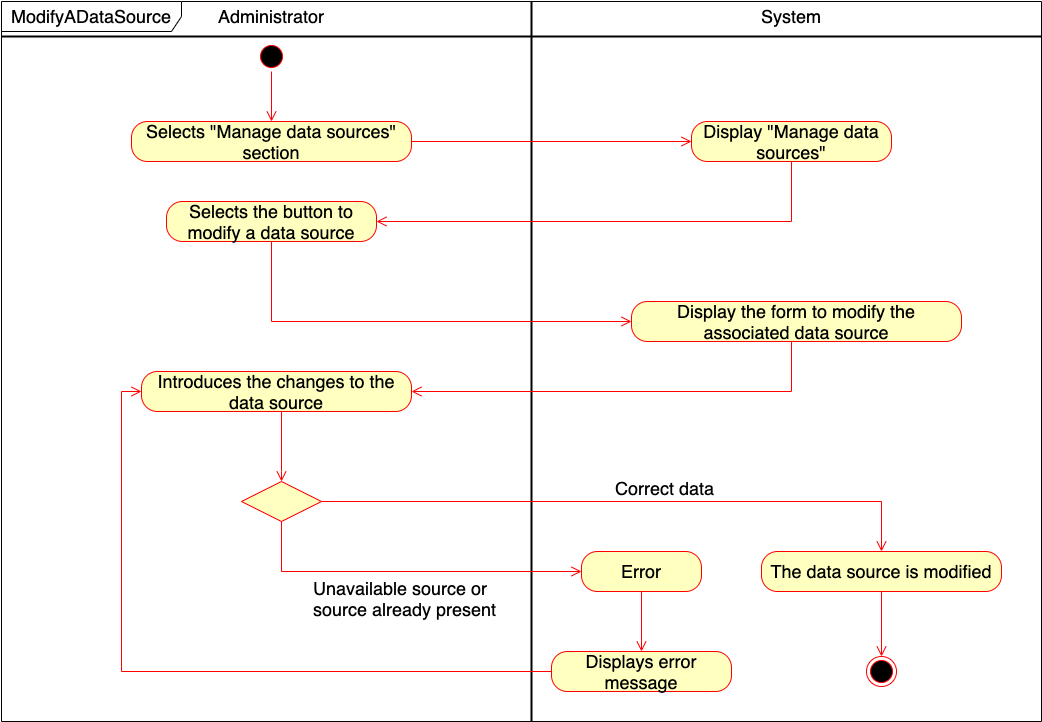
\includegraphics[scale=0.35]{images/use_cases_diagram/administrator_modify_datasource.png}
        \caption{Modify a data source}
        \label{fig:administrator_modify_datasource}
    \end{figure}
    \FloatBarrier
   
    \begin{longtable}{p{.25\textwidth} | p{.75\textwidth}}
     \caption{Remove a data source}
        \label{tab:remove_data_source}\\
        
        \hline
        \textbf{ID} & 22\\
        \hline
        \textbf{Name}  &  Remove a data source\\
        \hline
        \textbf{Actor}  &  Administrator\\
        \hline
        \textbf{Input}  &  Data source to remove\\
        \hline
        \textbf{Entry condition}  &  
        \begin{itemize}
                \item The Administrator is already registered in the system
                \item The Administrator is already logged in the system
                \item The Administrator is in the admin home page
         \end{itemize}\\
        \hline
        \textbf{Events flow} & 
        \begin{itemize}
                \item The Administrator selects the “Data sources” section
                \item The System opens the “Data sources” page
                \item The Administrator clicks on the button to remove a data source, associated to the data source he wants to remove
                \item The System render an alert asking for confirmation to remove the data source
                \item The Administrator confirms the operation 
                 \end{itemize}
                 \\
        \hline
        \textbf{Exit condition} & The data source is no more available in the system\\
        \hline
        \textbf{Exceptions} &  The Administrator doesn’t confirm the operation\\
        \hline
       
       
    \end{longtable}
    
    \begin{figure}[h!]
        \centering
        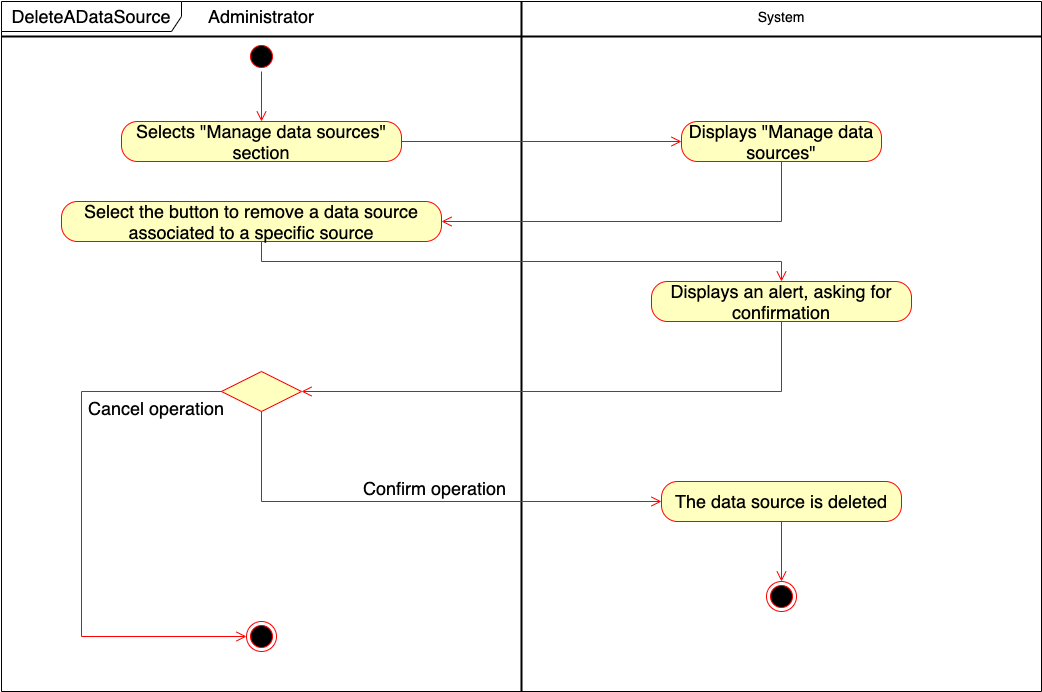
\includegraphics[scale=0.35]{images/use_cases_diagram/administrator_delete_datasource.png}
        \caption{Remove a data source}
        \label{fig:administrator_remove_datasource}
    \end{figure}
 \FloatBarrier   
 
 \newpage